% Practice Test 17 — Oklahoma Edition
% Questions: 30 (19 MC + 11 SA)
% Generated by scripts/generate_practice_tests.py

\begin{practiceQuestion}{1-3-q27}{gmc}
\begin{questionText}
The table below shows a proportional relationship between gallons of gas and miles driven. What is $k$ and what does it mean?

\begin{center}
\begin{tabular}{|c|c|}
\hline
\textbf{Gallons ($x$)} & \textbf{Miles ($y$)} \\ \hline
$2$ & $54$ \\ \hline
$5$ & $135$ \\ \hline
$8$ & $216$ \\ \hline
\end{tabular}
\end{center}
\end{questionText}
\choiceA{$k = 2$; uses $2$ gallons per trip}
\choiceB{$k = 27$; drives $27$ miles per gallon}
\choiceC{$k = 54$; drives $54$ miles on $2$ gallons}
\choiceD{$k = 135$; drives $135$ miles on $5$ gallons}
\correctAnswer{B}
\explanation{$k = \frac{54}{2} = 27$, $\frac{135}{5} = 27$, $\frac{216}{8} = 27$. The car gets $27$ miles per gallon.}
\end{practiceQuestion}

\begin{practiceQuestion}{1-6-q29}{gsa}
\begin{questionText}
The double number line below relates inches on a blueprint to actual feet. A hallway measures $3.5$ inches on the blueprint. What is the actual length?

\begin{center}
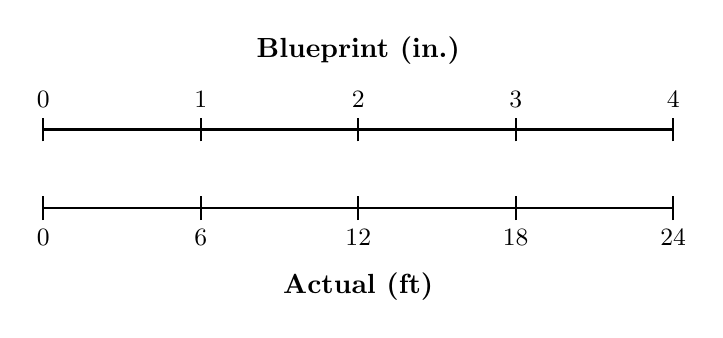
\begin{tikzpicture}[scale=1.0]
  % Top: blueprint inches
  \draw[thick] (0,1) -- (8,1);
  \foreach \x/\lab in {0/$0$, 2/$1$, 4/$2$, 6/$3$, 8/$4$} {
    \draw[thick] (\x,0.85) -- (\x,1.15);
    \node[above] at (\x,1.15) {\small \lab};
  }
  \node[above] at (4,1.7) {\textbf{Blueprint (in.)}};
  % Bottom: actual feet
  \draw[thick] (0,0) -- (8,0);
  \foreach \x/\lab in {0/$0$, 2/$6$, 4/$12$, 6/$18$, 8/$24$} {
    \draw[thick] (\x,-0.15) -- (\x,0.15);
    \node[below] at (\x,-0.15) {\small \lab};
  }
  \node[below] at (4,-0.7) {\textbf{Actual (ft)}};
\end{tikzpicture}
\end{center}
\end{questionText}
\correctAnswer{$21$ feet}
\explanation{Scale: $1$ inch $= 6$ feet. For $3.5$ inches: $6 \times 3.5 = 21$ feet.}
\end{practiceQuestion}

\begin{practiceQuestion}{1-7-q30}{gsa}
\begin{questionText}
The diagram shows a model and the real object with their measurements. Find the scale of the model.

\begin{center}
\begin{tikzpicture}[scale=0.7]
  % Model
  \draw[thick,funBlue,fill=funBlue!15] (0,0) rectangle (2,1.2);
  \node at (1,0.6) {Model};
  \draw[<->] (0,-0.3) -- (2,-0.3) node[midway,below] {$16$ cm};

  % Arrow
  \node at (3.5,0.6) {$\longrightarrow$};

  % Actual
  \draw[thick,funRed,fill=funRed!15] (5,0) rectangle (8.5,2.5);
  \node at (6.75,1.25) {Actual};
  \draw[<->] (5,-0.3) -- (8.5,-0.3) node[midway,below] {$40$ m};
\end{tikzpicture}
\end{center}
\end{questionText}
\correctAnswer{$1 : 250$}
\explanation{Convert: $40$ m $= 4{,}000$ cm. Divide: $4{,}000 \div 16 = 250$. The scale is $1 : 250$.}
\end{practiceQuestion}

\begin{practiceQuestion}{2-1-q04}{mc}
\begin{questionText}
A class has $32$ students. If $75\%$ passed the test, how many students passed?
\end{questionText}
\choiceA{$20$}
\choiceB{$24$}
\choiceC{$25$}
\choiceD{$28$}
\correctAnswer{B}
\explanation{$75\% = 0.75$. Multiply: $0.75 \times 32 = 24$ students passed.}
\end{practiceQuestion}

\begin{practiceQuestion}{2-4-q16}{mc}
\begin{questionText}
A bakery buys flour for $\$5$ per bag and sells muffins made from one bag for $\$20$. What is the percent markup on the flour cost?
\end{questionText}
\choiceA{$75\%$}
\choiceB{$150\%$}
\choiceC{$200\%$}
\choiceD{$300\%$}
\correctAnswer{D}
\explanation{Markup amount: $20 - 5 = 15$. Percent markup: $15 \div 5 = 3.00 = 300\%$.}
\end{practiceQuestion}

\begin{practiceQuestion}{2-7-q12}{mc}
\begin{questionText}
Two students estimated the number of beans in a jar. The actual count was $200$. Student A guessed $180$; Student B guessed $220$. Who had the greater percent error?
\end{questionText}
\choiceA{Student A}
\choiceB{Student B}
\choiceC{Same percent error}
\choiceD{Cannot be determined}
\correctAnswer{C}
\explanation{A: $\frac{|180-200|}{200} = 10\%$. B: $\frac{|220-200|}{200} = 10\%$. Both have $10\%$ error.}
\end{practiceQuestion}

\begin{practiceQuestion}{2-8-q02}{mc}
\begin{questionText}
You charge $\$300$ on a credit card with an $18\%$ annual interest rate. If you pay it off after $1$ year, how much interest do you owe?
\end{questionText}
\choiceA{$\$18$}
\choiceB{$\$36$}
\choiceC{$\$54$}
\choiceD{$\$318$}
\correctAnswer{C}
\explanation{Interest $= 300 \times 0.18 \times 1 = \$54$.}
\end{practiceQuestion}

\begin{practiceQuestion}{3-1-q23}{sa}
\begin{questionText}
Find two integers whose absolute values are both $7$.
\end{questionText}
\correctAnswer{$7$ and $-7$}
\explanation{$|7| = 7$ and $|-7| = 7$. A number and its opposite share the same absolute value.}
\end{practiceQuestion}

\begin{practiceQuestion}{4-1-q06}{mc}
\begin{questionText}
What is the value of $\frac{x}{2} - 4$ when $x = 10$?
\end{questionText}
\choiceA{$3$}
\choiceB{$-1$}
\choiceC{$1$}
\choiceD{$9$}
\correctAnswer{C}
\explanation{Substitute: $\frac{10}{2} - 4 = 5 - 4 = 1$.}
\end{practiceQuestion}

\begin{practiceQuestion}{4-2-q21}{sa}
\begin{questionText}
Simplify $-2a + 5b + 7a - 3b$.
\end{questionText}
\correctAnswer{$5a + 2b$}
\explanation{Combine $a$-terms: $-2a + 7a = 5a$. Combine $b$-terms: $5b - 3b = 2b$. Result: $5a + 2b$.}
\end{practiceQuestion}

\begin{practiceQuestion}{5-3-q15}{mc}
\begin{questionText}
Three friends split the cost of a gift equally. Each person also pays $\$4$ for wrapping. Each person pays $\$16$ total. What is the cost $c$ of the gift?
\end{questionText}
\choiceA{$c = 48$}
\choiceB{$c = 36$}
\choiceC{$c = 12$}
\choiceD{$c = 60$}
\correctAnswer{B}
\explanation{Each pays $\frac{c}{3} + 4 = 16$. This means $\frac{c}{3} = 12$, so $c = 36$. Or: total paid $= 3 \times 16 = 48$, wrapping $= 3 \times 4 = 12$, gift $= 48 - 12 = 36$.}
\end{practiceQuestion}

\begin{practiceQuestion}{5-4-q22}{sa}
\begin{questionText}
Solve $-0.3x + 4.2 = 1.8$.
\end{questionText}
\correctAnswer{$x = 8$}
\explanation{Subtract $4.2$: $-0.3x = -2.4$. Divide by $-0.3$: $x = 8$. Check: $-0.3(8) + 4.2 = -2.4 + 4.2 = 1.8$ \checkmark.}
\end{practiceQuestion}

\begin{practiceQuestion}{5-5-q30}{gsa}
\begin{questionText}
The table shows ticket prices for groups. A school has $\$200$ to spend and must also pay a $\$35$ bus fee. Write and solve an inequality to find the maximum number of students $s$ who can go.

\begin{center}
\begin{tabular}{|c|c|}
\hline
\textbf{Group Size} & \textbf{Price per Student} \\
\hline
$1$--$10$ & $\$12$ \\
\hline
$11$--$25$ & $\$9$ \\
\hline
$26+$ & $\$7$ \\
\hline
\end{tabular}
\end{center}

Assume the group qualifies for the $\$9$ rate.
\end{questionText}
\correctAnswer{$9s + 35 \leq 200$; $s \leq 18$}
\explanation{Total cost: $9s + 35 \leq 200$. Subtract $35$: $9s \leq 165$. Divide by $9$: $s \leq 18.\overline{3}$. Since $s$ must be a whole number, $s \leq 18$.}
\end{practiceQuestion}

\begin{practiceQuestion}{5-6-q24}{sa}
\begin{questionText}
What inequality is shown by a closed circle at $-6$ with shading to the right?
\end{questionText}
\correctAnswer{$x \geq -6$}
\explanation{Closed circle means $-6$ is included, shading right means values greater than or equal to $-6$: $x \geq -6$.}
\end{practiceQuestion}

\begin{practiceQuestion}{6-2-q05}{mc}
\begin{questionText}
When you redraw a scale drawing at a smaller scale (more real units per cm), the new drawing is:
\end{questionText}
\choiceA{Larger than the original drawing}
\choiceB{Smaller than the original drawing}
\choiceC{The same size as the original drawing}
\choiceD{A different shape than the original drawing}
\correctAnswer{B}
\explanation{A smaller scale means each cm represents more real distance, so fewer cm are needed. The drawing gets smaller. The shape stays the same.}
\end{practiceQuestion}

\begin{practiceQuestion}{6-3-q06}{mc}
\begin{questionText}
You know all three angles of a triangle: $50°$, $60°$, and $70°$. How many triangles can be drawn?
\end{questionText}
\choiceA{None}
\choiceB{Exactly one}
\choiceC{Exactly three}
\choiceD{More than one (infinitely many)}
\correctAnswer{D}
\explanation{Three angles (AAA) determine the shape but not the size. You can draw infinitely many similar triangles of different sizes with these angles.}
\end{practiceQuestion}

\begin{practiceQuestion}{6-4-q06}{mc}
\begin{questionText}
Two angles of a triangle are $35°$ and $75°$. What is the third angle?
\end{questionText}
\choiceA{$60°$}
\choiceB{$70°$}
\choiceC{$80°$}
\choiceD{$110°$}
\correctAnswer{B}
\explanation{$180° - 35° - 75° = 70°$.}
\end{practiceQuestion}

\begin{practiceQuestion}{6-5-q10}{mc}
\begin{questionText}
A cube can be sliced to produce a hexagonal cross-section. How?
\end{questionText}
\choiceA{By cutting parallel to the base}
\choiceB{By cutting diagonally through all six faces}
\choiceC{By cutting vertically through the center}
\choiceD{It is impossible to get a hexagon from a cube}
\correctAnswer{B}
\explanation{A diagonal plane that passes through all six faces of a cube creates a regular hexagonal cross-section.}
\end{practiceQuestion}

\begin{practiceQuestion}{6-6-q20}{sa}
\begin{questionText}
Find the supplement of $43°$.
\end{questionText}
\correctAnswer{$137°$}
\explanation{$180° - 43° = 137°$.}
\end{practiceQuestion}

\begin{practiceQuestion}{7-4-q04}{mc}
\begin{questionText}
A shape is made of a square with side $8$ cm and a semicircle with diameter $8$ cm attached to one side. What is the area? Use $\pi \approx 3.14$.
\end{questionText}
\choiceA{$64$ cm$^2$}
\choiceB{$89.12$ cm$^2$}
\choiceC{$114.24$ cm$^2$}
\choiceD{$139.12$ cm$^2$}
\correctAnswer{B}
\explanation{Square: $8^2 = 64$ cm$^2$. Semicircle: $\frac{1}{2} \times \pi r^2 = \frac{1}{2} \times 3.14 \times 16 = 25.12$ cm$^2$. Total: $64 + 25.12 = 89.12$ cm$^2$.}
\end{practiceQuestion}

\begin{practiceQuestion}{7-5-q17}{mc}
\begin{questionText}
A paint company needs to paint the outside of a box that is $3$ m by $2$ m by $1$ m. Each can of paint covers $5$ m$^2$. How many cans are needed?
\end{questionText}
\choiceA{$3$}
\choiceB{$4$}
\choiceC{$5$}
\choiceD{$6$}
\correctAnswer{C}
\explanation{$SA = 2(3 \times 2) + 2(3 \times 1) + 2(2 \times 1) = 12 + 6 + 4 = 22$ m$^2$. Cans: $22 \div 5 = 4.4$. Round up to $5$ cans.}
\end{practiceQuestion}

\begin{practiceQuestion}{7-6-q24}{sa}
\begin{questionText}
A planter box is $3$ ft long, $1.5$ ft wide, and $2$ ft deep. How many cubic feet of soil are needed to fill it?
\end{questionText}
\correctAnswer{$9$ ft$^3$}
\explanation{$V = 3 \times 1.5 \times 2 = 9$ ft$^3$.}
\end{practiceQuestion}

\begin{practiceQuestion}{8-1-q05}{mc}
\begin{questionText}
A random sample means that:
\end{questionText}
\choiceA{Only the best members are chosen}
\choiceB{The largest possible group is chosen}
\choiceC{Every member of the population has an equal chance of being selected}
\choiceD{Only volunteers are selected}
\correctAnswer{C}
\explanation{In a random sample, every member of the population has an equal chance of being chosen.}
\end{practiceQuestion}

\begin{practiceQuestion}{8-3-q25}{sa}
\begin{questionText}
Two groups have means of $50$ and $54$, and both have MAD $= 8$. Express the difference in means as a multiple of MAD. Is the difference meaningful?
\end{questionText}
\correctAnswer{$0.5$ MADs; no, the difference is not meaningful}
\explanation{$\frac{54-50}{8} = 0.5$ MADs. Since $0.5 < 2$, the difference is small relative to the variability and not considered meaningful.}
\end{practiceQuestion}

\begin{practiceQuestion}{8-4-q27}{gmc}
\begin{questionText}
The box plots show quiz scores (out of $20$) for two classes.

\begin{center}
\begin{tikzpicture}[scale=0.35]
  \draw[thick,->] (4,0) -- (21,0);
  \foreach \x in {5,6,...,20} {
    \draw (\x,0.3) -- (\x,-0.3);
    \node[below,font=\tiny] at (\x,-0.3) {$\x$};
  }
  % Class M: min=8, Q1=12, med=15, Q3=17, max=20
  \draw[thick] (8,3) -- (20,3);
  \draw[thick,fill=funBlue!30] (12,2) rectangle (17,4);
  \draw[very thick,funBlue] (15,2) -- (15,4);
  \draw[thick] (8,2) -- (8,4);
  \draw[thick] (20,2) -- (20,4);
  \node[right,font=\small] at (20.5,3) {Class M};
  % Class N: min=10, Q1=13, med=16, Q3=18, max=19
  \draw[thick] (10,7) -- (19,7);
  \draw[thick,fill=funGreen!30] (13,6) rectangle (18,8);
  \draw[very thick,funGreen] (16,6) -- (16,8);
  \draw[thick] (10,6) -- (10,8);
  \draw[thick] (19,6) -- (19,8);
  \node[right,font=\small] at (19.5,7) {Class N};
\end{tikzpicture}
\end{center}

What is the IQR for each class?
\end{questionText}
\choiceA{Class M: $5$, Class N: $5$}
\choiceB{Class M: $12$, Class N: $9$}
\choiceC{Class M: $5$, Class N: $9$}
\choiceD{Class M: $12$, Class N: $5$}
\correctAnswer{A}
\explanation{Class M: $Q_3 - Q_1 = 17 - 12 = 5$. Class N: $18 - 13 = 5$. Both have IQR $= 5$.}
\end{practiceQuestion}

\begin{practiceQuestion}{8-5-q29}{gsa}
\begin{questionText}
The stem-and-leaf plot shows the ages of people at a family reunion.

\begin{center}
\begin{tabular}{r|l}
\textbf{Stem} & \textbf{Leaf} \\
\hline
$0$ & $5\;\;8\;\;9$ \\
$1$ & $2\;\;4\;\;6$ \\
$2$ & $0\;\;5\;\;8$ \\
$3$ & $2\;\;5\;\;7\;\;9$ \\
$4$ & $1\;\;5$ \\
$5$ & $0\;\;8$ \\
$6$ & $3\;\;7$ \\
$7$ & $2$
\end{tabular}

Key: $3 \mid 2$ means $32$ years old
\end{center}

Find the range and median of the ages.
\end{questionText}
\correctAnswer{Range $= 67$; Median $= 33.5$}
\explanation{Data ($20$ values): $5, 8, 9, 12, 14, 16, 20, 25, 28, 32, 35, 37, 39, 41, 45, 50, 58, 63, 67, 72$. Range $= 72 - 5 = 67$. Median $= \frac{32+35}{2} = 33.5$.}
\end{practiceQuestion}

\begin{practiceQuestion}{8-7-q01}{mc}
\begin{questionText}
A frequency table lists:
\end{questionText}
\choiceA{Only the largest and smallest values}
\choiceB{Categories and how often each occurs}
\choiceC{The mean, median, and mode}
\choiceD{Data arranged in a circle}
\correctAnswer{B}
\explanation{A frequency table shows each category (or interval) and the count of data values in it.}
\end{practiceQuestion}

\begin{practiceQuestion}{9-4-q14}{mc}
\begin{questionText}
A student creates a probability model for a spinner: $P(\text{red}) = 0.25$, $P(\text{blue}) = 0.25$, $P(\text{green}) = 0.25$, $P(\text{yellow}) = 0.25$. After $200$ spins, the results are: red $= 55$, blue $= 48$, green $= 52$, yellow $= 45$. Is the model a good fit?
\end{questionText}
\choiceA{No, the model is completely wrong}
\choiceB{Yes, the observed frequencies are reasonably close to $50$ each}
\choiceC{No, because the results are not exactly $50$ each}
\choiceD{Yes, because $200$ is divisible by $4$}
\correctAnswer{B}
\explanation{Each color should appear about $50$ times ($200 \times 0.25$). The results ($55, 48, 52, 45$) are all close to $50$, supporting the model.}
\end{practiceQuestion}

\begin{practiceQuestion}{9-6-q27}{gmc}
\begin{questionText}
The tree diagram shows the outcomes for flipping two coins. What is the probability of getting at least one tail?

\begin{center}
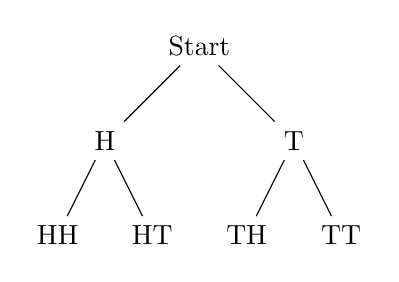
\begin{tikzpicture}[scale=0.8,
  level 1/.style={sibling distance=3cm, level distance=1.5cm},
  level 2/.style={sibling distance=1.5cm, level distance=1.5cm}]
  \node {Start}
    child {node {H}
      child {node {HH}}
      child {node {HT}}
    }
    child {node {T}
      child {node {TH}}
      child {node {TT}}
    };
\end{tikzpicture}
\end{center}
\end{questionText}
\choiceA{$\frac{1}{4}$}
\choiceB{$\frac{1}{2}$}
\choiceC{$\frac{3}{4}$}
\choiceD{$\frac{2}{4}$}
\correctAnswer{C}
\explanation{Outcomes with at least one tail: HT, TH, TT — that is $3$ out of $4$. $P = \frac{3}{4}$.}
\end{practiceQuestion}

\begin{practiceQuestion}{9-7-q27}{gmc}
\begin{questionText}
The bar graph shows the results of simulating a spinner $100$ times. The spinner is supposed to land on each color with equal probability. Based on the simulation, does the spinner appear fair?

\begin{center}
\begin{tikzpicture}[scale=0.55]
  \draw[thick,->] (0,0) -- (0,32) node[above,font=\small] {Frequency};
  \draw[thick,->] (0,0) -- (7,0);
  \foreach \y in {5,10,...,30} {
    \draw[gray!30] (0,\y) -- (6.5,\y);
    \node[left,font=\small] at (0,\y) {\y};
  }
  \fill[funRed!70] (0.5,0) rectangle (1.5,26);
  \fill[funBlue!70] (2.5,0) rectangle (3.5,24);
  \fill[funGreen!70] (4.5,0) rectangle (5.5,28);
  \node[below,font=\small] at (1,0) {Red};
  \node[below,font=\small] at (3,0) {Blue};
  \node[below,font=\small] at (5,0) {Grn.};
  \node[below,font=\small] at (3,-1) {Not shown: Yellow $= 22$};
\end{tikzpicture}
\end{center}
\end{questionText}
\choiceA{No, because the bars are different heights}
\choiceB{Yes, the frequencies ($26, 24, 28, 22$) are all roughly close to $25$}
\choiceC{No, Green is clearly the most likely color}
\choiceD{Cannot be determined from the graph}
\correctAnswer{B}
\explanation{With $4$ equal sections, each should appear about $25$ times in $100$ spins. The results ($26, 24, 28, 22$) are all close to $25$, suggesting the spinner is fair.}
\end{practiceQuestion}
